\documentclass[a4paper, 12pt]{article}

\usepackage{graphicx}
\usepackage{xcolor}
\usepackage{mdframed}
\usepackage { amsmath , amssymb , amsthm }
\usepackage[T2A]{fontenc}
\usepackage[utf8]{inputenc}
\usepackage[english,russian]{babel}

\graphicspath{{img/}}
\DeclareGraphicsExtensions{.pdf,.png,.jpg}


\title{Инженерная графика}
\author{Щербинин В.В}
\date{\today}

\begin{document}
\maketitle

\section*{Введение}

ЕСКД -- единая система конструкторской документации (устанавливает взаимосвязь правил по оформлению, конструированию, обращинию конструкторской документации)\\
"+":\\
1. Возможность взаимообмена конструкторской документации между предприятиями.\\
2. Стабилизация комплектности, исключающая дубрированость документов.\\
3. Возможность обеспечивать унификации при конструировании, разработке, проэктированиии комерческих изделий\\
4. Упращенная форма конструкторской документации.\\
5. Механизм и автоматизм обработки технической документации.\\
\newpage
\section{Методы проекции}

\subsection{Центральная проекция}
Для получения центральных проекций необходимо задаться плоскостью проекций H и центром проекций S.\\
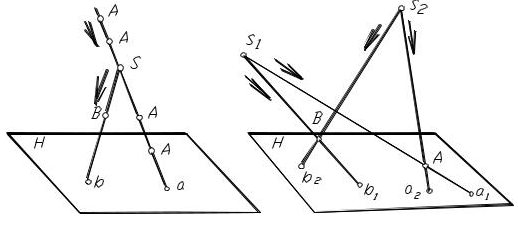
\includegraphics{eng1}\\
Центр проекций действует как точечный источник света, испуская проецирующие лучи. Точки пересечения проецирующих лучей с плоскостью проекций H называются проекциями. Проекций не получается, когда центр проецирования лежит в данной плоскости или проецирующие лучи параллельны плоскости проекций.\\

Свойства центрального проецирования:\\
1.Каждая точка пространства проецируется на данную плоскость проекций в единственную проекцию.\\
2.В то же время каждая точка на плоскости проекций может быть проекцией множества точек, если они находятся на одном проецирующем луче\\
3.Прямая, не проходящая через центр проецирования, проецируется прямой (проецирующая прямая – точкой).\\
4.Плоская (двумерная) фигура, не принадлежащая проецирующей плоскости, проецируется двумерной фигурой (фигуры, принадлежащие проецирующей плоскости, проецируются вместе с ней в виде прямой).\\
5.Трехмерная фигура отображается двумерной.\\
Глаз, фотоаппарат являются примерами этой системы изображения. Одна центральная проекция точки не дает возможность судить о положении самой Точки в пространстве, и поэтому в техническом черчении это проецированиепочти не применяется. Для определения положения точки при данном способе необходимо иметь две ее центральные проекции, полученные из двух различных центров. Центральные проекции применяют для изображения предметов в перспективе. Изображения в центральных проекциях наглядны, но для технического черчения неудобны.

\subsection{Параллельная проекция и их свойства}
Параллельное проецирование – частный случай центрального проецирования, когда центр проецирования перемещен в несобственную точку, т.е. в бесконечность. При таком положении центра проекций все проецирующие прямые будут параллельны между собой. В связи с параллельностью проецирующих прямых рассматриваемый способ называется параллельным, а полученные с его помощью проекции – параллельными проекциями. Аппарат параллельного проецирования полностью определяется положением плоскости проецирования (H) и направлением проецирования.\\

Свойства параллельного проецирования:\\
1.При параллельном проецировании сохраняются все свойства центрального проецирования, а также возникают новые:\\
2.Для определения положения точки в пространстве необходимо иметь две ее параллельные проекции, полученные при двух различных направлениях проецирования.\\
3.Параллельные проекции взаимно параллельных прямых параллельны, а отношение длин отрезков таких прямых равно отношению длин их проекций.\\
4.Если длина отрезка прямой делится точкой в каком-либо отношении, то и длина проекции отрезка делится проекцией этой точки в том же отношении .\\
5.Плоская фигура, параллельная плоскости проекций , проецируется при параллельном проецировании на эту плоскость в такую же фигуру.\\

Параллельное проецирование, как и центральное, при одном центре проецирования, также не обеспечивает обратимости чертежа.\\
Применяя приемы параллельного проецирования точки и линии, можно строить параллельные проекции поверхности и тела.\\

\subsection{Прямоугольное (ортогональное)проецирование}

\end{document}